\chapter{Rezultati}
V tem poglavju bom opisal rezultate, ki sem jih pridobil. Kot sem že omenil, bo večji del preizkušanja programa opravljen na slikah, kjer bodo nekateri piksli manjkali. Gre za problem, ki ga je moč lepo vizualizirati, saj pogosto pri surovih podatkih ni lahko definirati njihovo točnost, zaradi česar težko interpretiramo, kako koristen je sam algoritem.

Prav tako bom opisal točnost rezulatov različnih metod kot tudi čas izvajanja posameznih metod. Probleme bom zagnal tudi na različnih vrst podatkov, npr. podatkih ki so generirani normalno kot tudi enakomerno porazdeljeno.

Poglavje bom začel pisati, ko končam z vsemi implementacijami, pri delu pa si bom pomagal z orodjem Microsoft Excel, kjer bom lahko napake in čas izvajanja tudi grafično vizualiziral. 

Zaradi interpretacije, sem slike razdelil v več skupin, za katere opišemo ugotovitve.

\section{Velika črno-bela slika}
Same teste algoritmov najprej poženemo na veliki, črno-beli sliki, velikosti $1000\times1000$ pikslov. Taka izbira je smiselna, iz vidika, da imamo dovolj podatkov, potrebnih za rekonstrukcijo. Ker je časovna zahtevnost algoritmov pri večjih slikah, kot bomo videli v nadaljevanju že precej velika, nam ta faza testiranja služi kot preverjanje delovanja samih algoritmov. Same podrobnosti razlik med rezultati si bomo zato podrobneje pogledali na manjših slikah v nadaljevanju. Algoritme preizkušamo trikrat, na podatkih z deleži znanih vrednosti $0.35, 0.45$ in $0.6$.
\begin{figure}[h]
    \centering
    \begin{subfigure}{0.49\linewidth}
        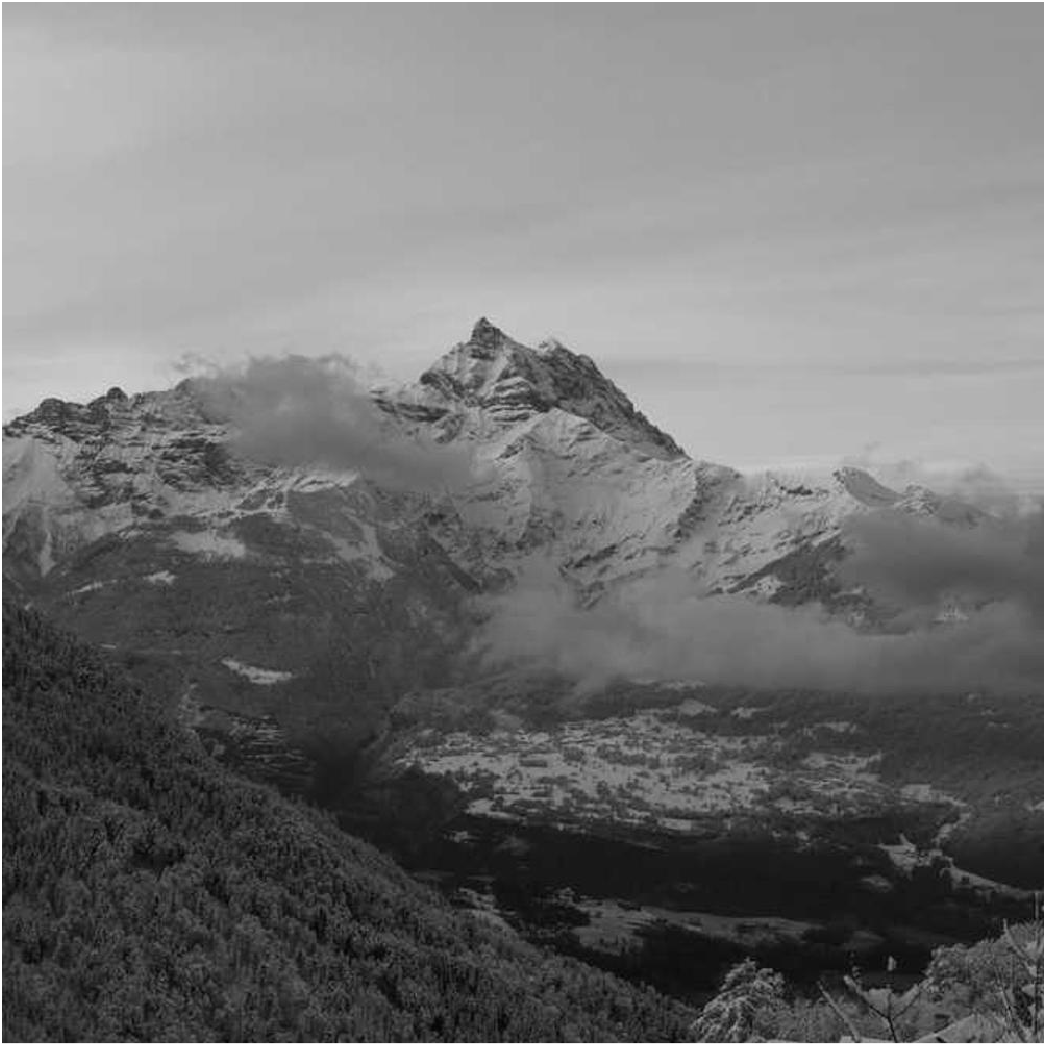
\includegraphics[width=\linewidth]{Poglavja/Slike/grayscale1000/slikaInput.png}
        \caption{Originalna slika}
    \end{subfigure}
    \hfill
    \begin{subfigure}{0.49\linewidth}
        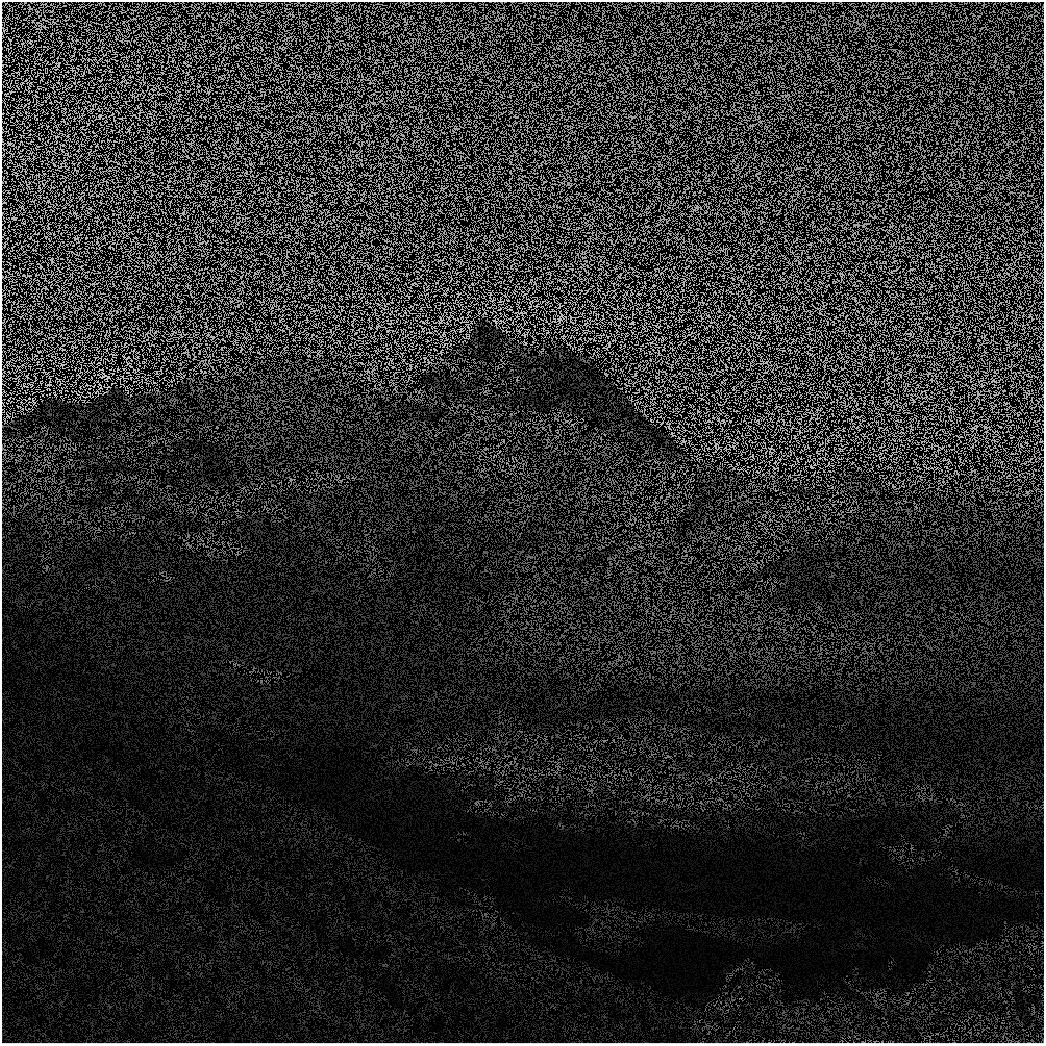
\includegraphics[width=\linewidth]{Poglavja/Slike/grayscale1000/slikaInput35.png}
        \caption{Slika z $0.35$ znanimi podatki}
    \end{subfigure}
    \begin{subfigure}{0.49\linewidth}
        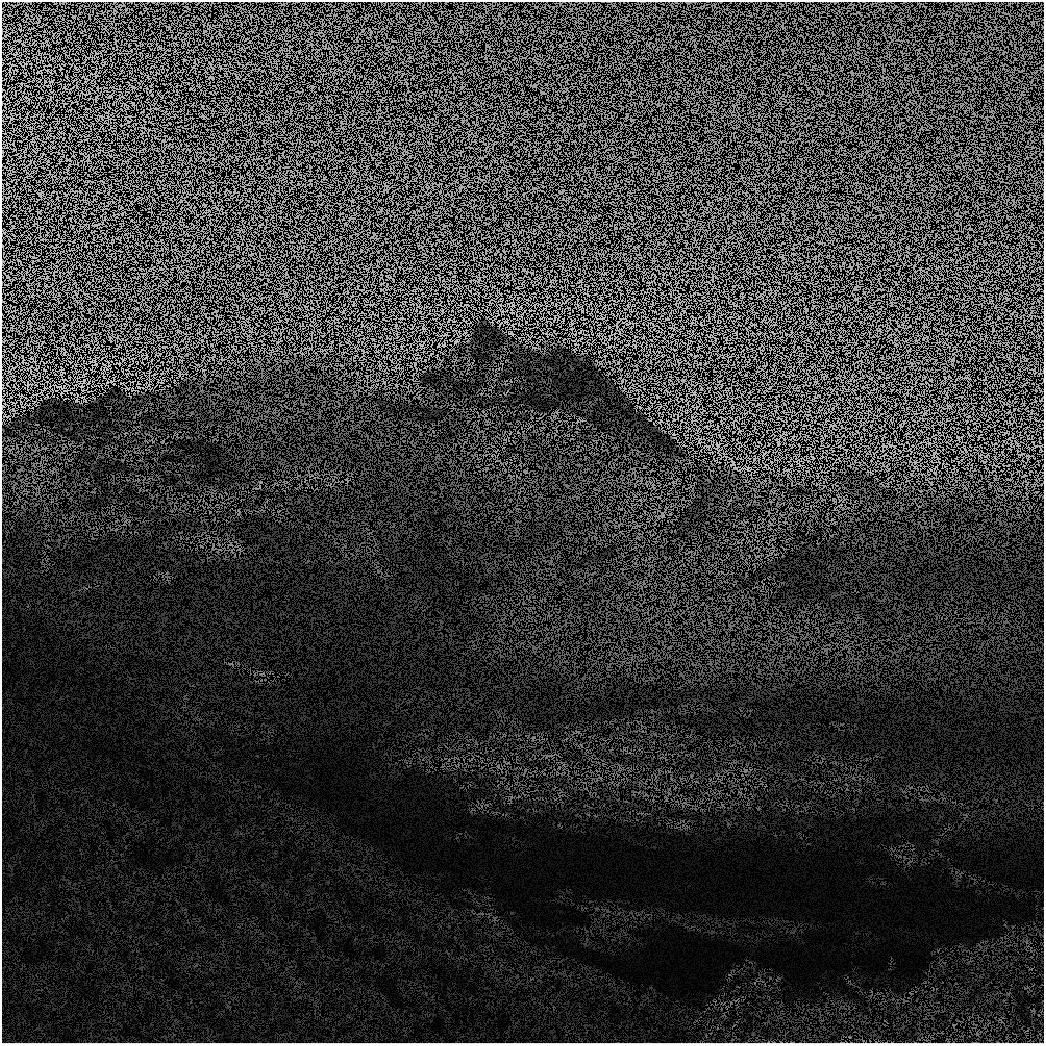
\includegraphics[width=\linewidth]{Poglavja/Slike/grayscale1000/slikaInput45.png}
        \caption{Slika z $0.45$ znanimi podatki}
    \end{subfigure}
    \hfill
    \begin{subfigure}{0.49\linewidth}
        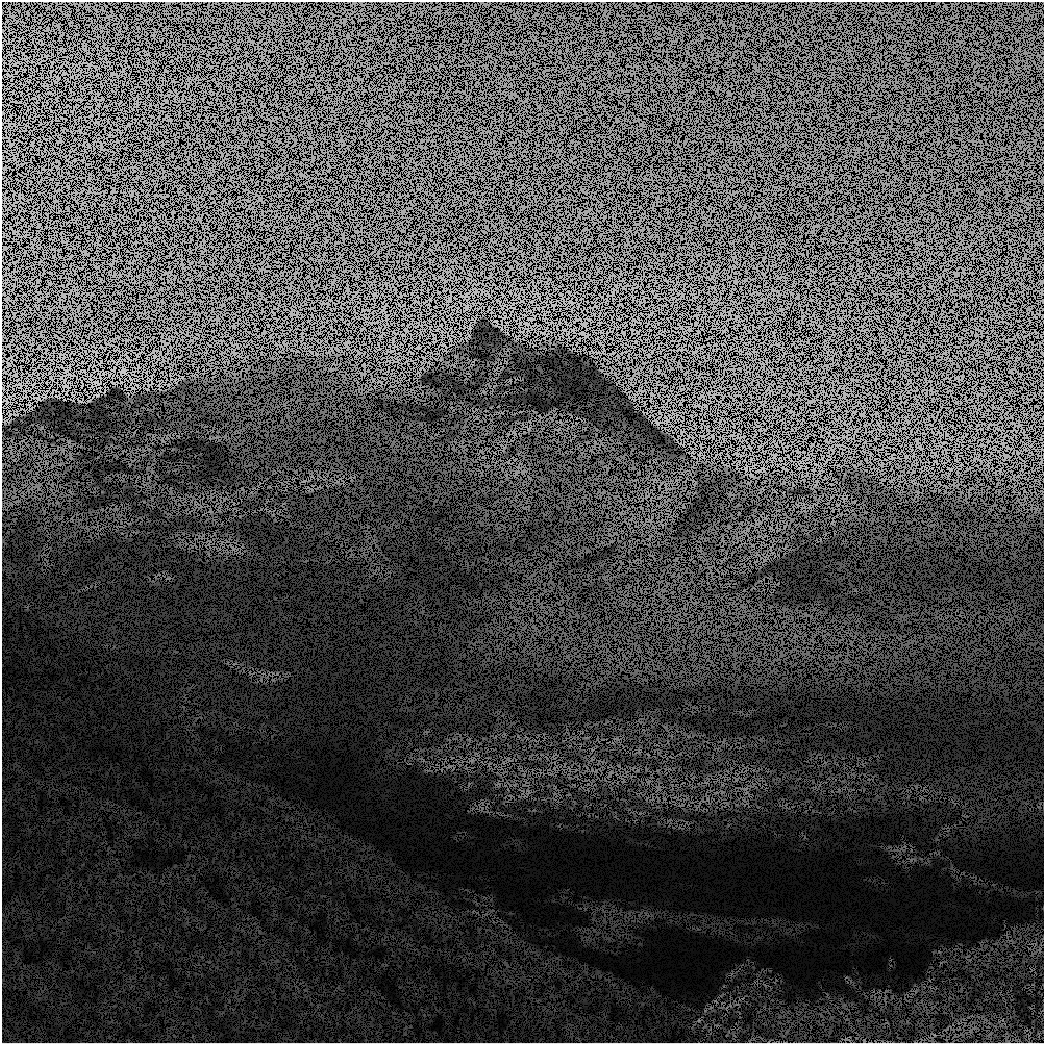
\includegraphics[width=\linewidth]{Poglavja/Slike/grayscale1000/slikaInput60.png}
        \caption{Slika z $0.60$ znanimi podatki}
    \end{subfigure}
    \caption{Vir slike: Unsplash}
\end{figure}

Kot vidimo, je med rezultati velika razlika. Očitno je, da algoritma TNNM in SVT delujeta najbolje, medtem ko imata algoritma ADDM in LMaFit vprašljive rezultate. Te si lahko interpretiramo kot posledica slabosti, da lahko algoritma končata v lokalnem optimumu. Zato je ta algoritma smiselno uporabljati, kadar ima dober začeten približek matrik $X$ in $Y$. Algoritem NNM med rezultati manjka, saj je zaradi velikega števila matrik, potrebnih za definicijo omejitev, algoritem preveč prostorsko kompleksen. Ta algoritem bomo zato obravnavali posebej.